
%%%%%%%%%%%%%%%%%%%%%%%%%%%%%%%%%%%%%%%%%%%%%%%%%%%%%%%%%%%%%%%%%%%%%%%
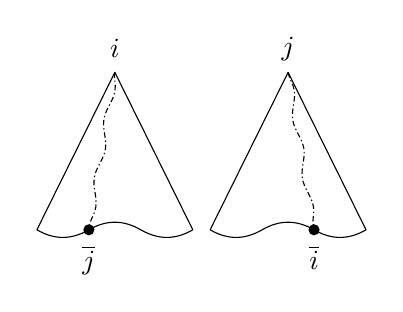
\begin{tikzpicture}[
edge from parent path=,
level distance=2cm,
level/.style={sibling distance=0.66cm/#1}
%,scale=1, every node/.style={transform shape}
]

  \tikzstyle{ref}=[circle,fill=black,inner sep=0.5mm]
  \tikzstyle{dashdot}=[dashed,dash pattern=on 2pt off 1pt on 0.5pt off 1pt]
  \tikzstyle{mysnake}=[decorate,decoration={snake,amplitude=0.4mm,segment length=0.75cm}]

  \node (c11) {}
    child { node (c12) {} }
    child { node (c13) [ref,label={below:$\overline{j}$}] {} }
    child { node (c14) {} }
    child { node (c15) {} };

  \node (c10) [minimum height=0.5cm,node distance=0.3cm,above of=c11] {$i$};

  \draw [join=round] (c11.center)
     to (c12.center) 
     to [bend right] (c13.center)
     to [bend left] (c14.center)
     to [bend right] (c15.center)
     -- cycle;

  \draw [mysnake,dashdot] (c11.center) -- (c13.center);

  \node (c21) [node distance=2.2cm,right of=c11] {}
    child { node (c22) {} }
    child { node (c23) {} }
    child { node (c24) [ref,label={below:$\overline{i}$}] {} }
    child { node (c25) {} };

  \node (c20) [minimum height=0.5cm,node distance=0.3cm,above of=c21] {$j$};

  \draw [join=round] (c21.center)
    to (c22.center) 
    to [bend right] (c23.center)
    to [bend left] (c24.center)
    to [bend right] (c25.center)
    -- cycle;

  \draw [mysnake,dashdot] (c21.center) -- (c24.center);

\end{tikzpicture}
